
\section{Injektivität, Surjektivität und Bijektivität von Abbildungen}

\subsection{Injektivität von Abbildungen}

\textbf{Definition (injektiv):}\\
Eine Abb. $f:\mathbb{D}_f\longmapsto\mathbb{W}_f$ heißt injektiv, wenn $f(x_1)=f(x_2)$ nur für $x_1=x_2$ gilt.\\
Beispiel:\\
$f_2:\mathbb{R}\longmapsto[0,\infty[$ mit $x\longmapsto x^2$\\
\textbullet \;\;Zeige, dass $f_2$ nicht injektiv ist.\\
\begin{quote}
	$f_2:\mathbb{R}\longmapsto [0,\infty[$ mit $x\longmapsto x^2$\\
	$ f_2(-1)=(-1)^2=1$\\
	$f_2(1)=(1)^2=1$\\
	es muß gelten:\\
	$f_2(x_1)=f(x_2)$ nur für $x_1=x_2$\\
	Widerspruchsbeweis:\\
	Für $x_1=-1$ gilt $f(x_1)=1$ und für $x_2=1$ gilt $f_2(x_2)=1\Rightarrow x_1\neq x_2\wedge f(x_1)=f(x_2).\\\text{Widerspruch zur Definition} \Rightarrow f_2(x) \text{ ist nicht injektiv.}_{\Square} $ \\ 
	
\end{quote}

\begin{center}
	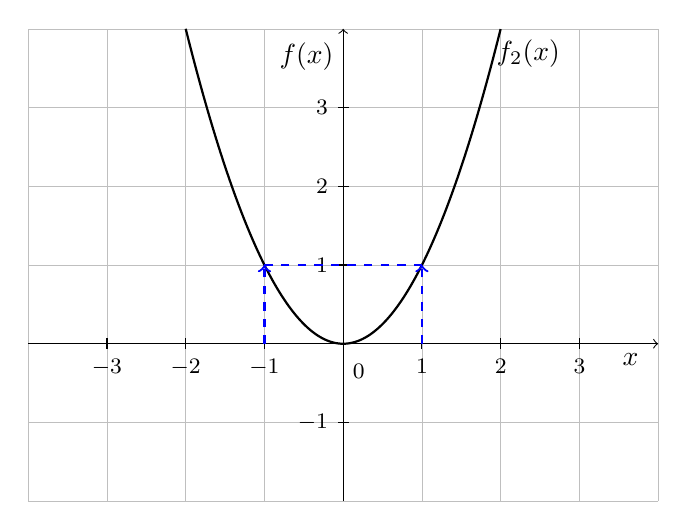
\begin{tikzpicture}
		
		% Gitternetzlinien
		\draw[xstep=1cm, ystep=1cm, very thin, color=lightgray] (-4,4) grid (4,-2);
		% x-Achse
		\draw[->] (-4,0) -- (4,0) node[below,xshift=-1em] {$x$}; 
		%Zahlen auf x-Achse
		\foreach \x in {-3,...,-1}
		\draw[shift={(\x,0)},color=black] (0pt,2pt) -- (0pt,-2pt) node[below] {\footnotesize $\x$};
		\foreach \x in {1,...,3}
		\draw[shift={(\x,0)},color=black] (0pt,2pt) -- (0pt,-2pt) node[below] {\footnotesize $\x$};
		% y-Achse 
		\draw[->] (0,-2) -- (0,4) node[left,yshift=-1em] {$f(x)$};%node[above left]
		%Zahlen auf y-Achse
		\foreach \y in {-1,...,-1}
		\draw[shift={(0,\y)},color=black] (2pt,0pt) -- (-2pt,0pt) node[left] {\footnotesize $\y$};
		\foreach \y in {1,...,3}
		\draw[shift={(0,\y)},color=black] (2pt,0pt) -- (-2pt,0pt) node[left] {\footnotesize $\y$};
		%Ursprung
		\draw[color=black] (0pt,-10pt) node[right] {\footnotesize $0$};
		
		
		
		\draw[thick,color=black] plot[samples=200, domain=-2:2] 
		(\x,{\x*\x}) node[below, xshift=1em]{$f_2(x)$};
		
		\draw[color=blue,thick,dashed] (-1,1) -- (1,1);
		\draw[->,color=blue,thick,dashed] (-1,0) -- (-1,1);
		\draw[->,color=blue,thick,dashed] (1,0) -- (1,1);
		
	\end{tikzpicture}\\
\end{center}
\newpage
\noindent
\textbullet \;\; $f_{2_{|[0,\infty[}}$  ist injektiv .\\
\begin{center}
	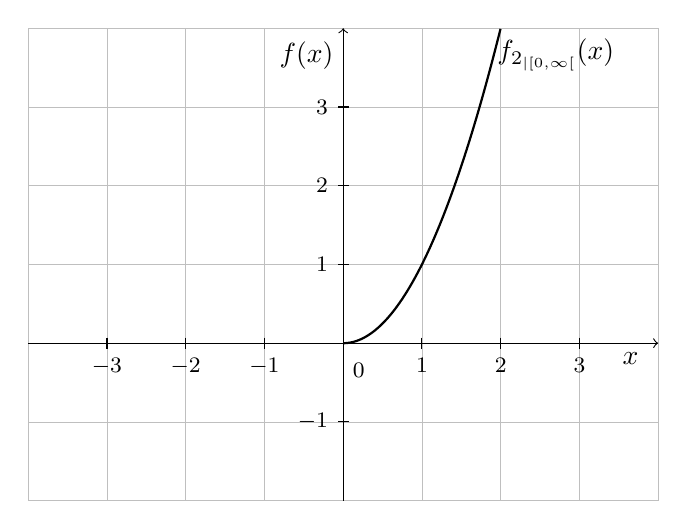
\begin{tikzpicture}
		
		% Gitternetzlinien
		\draw[xstep=1cm, ystep=1cm, very thin, color=lightgray] (-4,4) grid (4,-2);
		% x-Achse
		\draw[->] (-4,0) -- (4,0) node[below,xshift=-1em] {$x$}; 
		%Zahlen auf x-Achse
		\foreach \x in {-3,...,-1}
		\draw[shift={(\x,0)},color=black] (0pt,2pt) -- (0pt,-2pt) node[below] {\footnotesize $\x$};
		\foreach \x in {1,...,3}
		\draw[shift={(\x,0)},color=black] (0pt,2pt) -- (0pt,-2pt) node[below] {\footnotesize $\x$};
		% y-Achse 
		\draw[->] (0,-2) -- (0,4) node[left,yshift=-1em] {$f(x)$};%node[above left]
		%Zahlen auf y-Achse
		\foreach \y in {-1,...,-1}
		\draw[shift={(0,\y)},color=black] (2pt,0pt) -- (-2pt,0pt) node[left] {\footnotesize $\y$};
		\foreach \y in {1,...,3}
		\draw[shift={(0,\y)},color=black] (2pt,0pt) -- (-2pt,0pt) node[left] {\footnotesize $\y$};
		%Ursprung
		\draw[color=black] (0pt,-10pt) node[right] {\footnotesize $0$};
		
		
		
		\draw[thick,color=black] plot[samples=200, domain=0:2] 
		(\x,{\x*\x}) node[below, xshift=2em]{$f_{2_{|[0,\infty[}}(x)$};
		
		
		
	\end{tikzpicture}\\
\end{center}
\begin{quote}
	Merke: Die Injektivität hängt stark vom $ \mathbb{D}_f$ ab.
\end{quote}
\newpage
\noindent

Beispiel: $f(x)=2$\\
\begin{center}
	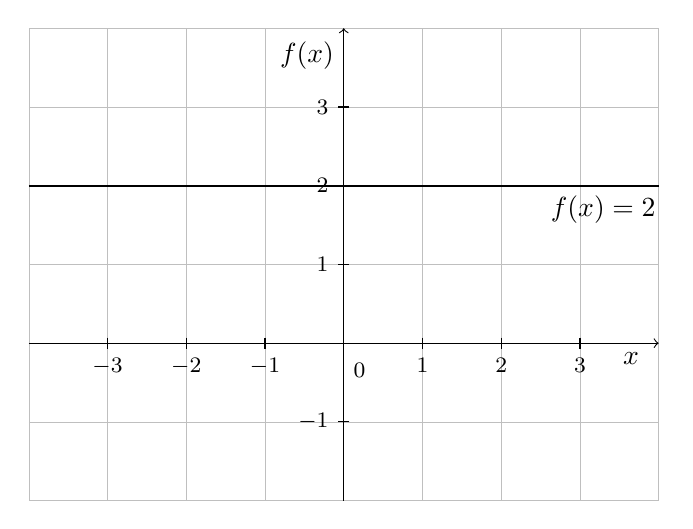
\begin{tikzpicture}
		
		% Gitternetzlinien
		\draw[xstep=1cm, ystep=1cm, very thin, color=lightgray] (-4,4) grid (4,-2);
		% x-Achse
		\draw[->] (-4,0) -- (4,0) node[below,xshift=-1em] {$x$}; 
		%Zahlen auf x-Achse
		\foreach \x in {-3,...,-1}
		\draw[shift={(\x,0)},color=black] (0pt,2pt) -- (0pt,-2pt) node[below] {\footnotesize $\x$};
		\foreach \x in {1,...,3}
		\draw[shift={(\x,0)},color=black] (0pt,2pt) -- (0pt,-2pt) node[below] {\footnotesize $\x$};
		% y-Achse 
		\draw[->] (0,-2) -- (0,4) node[left,yshift=-1em] {$f(x)$};%node[above left]
		%Zahlen auf y-Achse
		\foreach \y in {-1,...,-1}
		\draw[shift={(0,\y)},color=black] (2pt,0pt) -- (-2pt,0pt) node[left] {\footnotesize $\y$};
		\foreach \y in {1,...,3}
		\draw[shift={(0,\y)},color=black] (2pt,0pt) -- (-2pt,0pt) node[left] {\footnotesize $\y$};
		%Ursprung
		\draw[color=black] (0pt,-10pt) node[right] {\footnotesize $0$};
		
		
		
		\draw[thick,color=black] plot[samples=200, domain=-4:4] 
		(\x,{2}) node[below, xshift=-2em]{$f(x)=2$};
		
		
		
	\end{tikzpicture}\\
\end{center}
Diese Funktion ist nicht injektiv. Jedem Wert der $ x$-Achse wird ein Wert an der $y$-Achse zugewiesen.\vspace*{2mm}
\\
Beispiel: $f(x)=3\sin(x)+1$\\
\begin{center}
	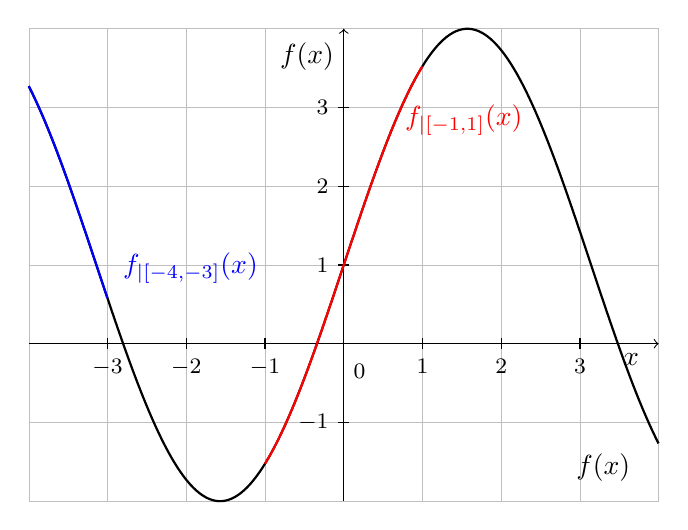
\begin{tikzpicture}
		
		% Gitternetzlinien
		\draw[xstep=1cm, ystep=1cm, very thin, color=lightgray] (-4,4) grid (4,-2);
		% x-Achse
		\draw[->] (-4,0) -- (4,0) node[below,xshift=-1em] {$x$}; 
		%Zahlen auf x-Achse
		\foreach \x in {-3,...,-1}
		\draw[shift={(\x,0)},color=black] (0pt,2pt) -- (0pt,-2pt) node[below] {\footnotesize $\x$};
		\foreach \x in {1,...,3}
		\draw[shift={(\x,0)},color=black] (0pt,2pt) -- (0pt,-2pt) node[below] {\footnotesize $\x$};
		% y-Achse 
		\draw[->] (0,-2) -- (0,4) node[left,yshift=-1em] {$f(x)$};%node[above left]
		%Zahlen auf y-Achse
		\foreach \y in {-1,...,-1}
		\draw[shift={(0,\y)},color=black] (2pt,0pt) -- (-2pt,0pt) node[left] {\footnotesize $\y$};
		\foreach \y in {1,...,3}
		\draw[shift={(0,\y)},color=black] (2pt,0pt) -- (-2pt,0pt) node[left] {\footnotesize $\y$};
		%Ursprung
		\draw[color=black] (0pt,-10pt) node[right] {\footnotesize $0$};
		
		
		
		\draw[thick,color=black] plot[samples=200, domain=-4:4] 
		(\x,{3*sin(\x r)+1}) node[below, xshift=-2em]{$f(x)$};
		
		\draw[thick,color=blue] plot[samples=200, domain=-4:-3] 
		(\x,{3*sin(\x r)+1}) node[below, xshift=3em,yshift=2em]{$f_{|[-4,-3]}(x)$};
		\draw[thick,color=red] plot[samples=200, domain=-1:1] 
		(\x,{3*sin(\x r )+1}) node[below, xshift=1.5em,yshift=-1em]{$f_{|[-1,1]}(x)$};
		
	\end{tikzpicture}\\
\end{center}
Die Funktion $f(x)$ ist nicht injektiv. Durch Einschränkung der  Funktion $f(x)$ kann ein Teil injektiv werden. Die Funktion $f_{|[-4,-3]}(x)$ und $f_{|[-1,1]}(x)$ sind injektiv.\\
\subsection{Surjektivität und Bijektivität von Abbildungen}

\textbf{Definition (surjektiv):}\\
Eine Abbildung
$f:\mathbb{D}_f\rightarrow\mathbb{W}_f$
heißt surjektiv, wenn zu jedem Element
$y$ der Zielmenge mindestens ein Element
$x$ des Definitionsbereichs existiert,
sodass $f(x)=y$ gilt.

Mathematisch:

\begin{align*}
	\forall y\in\mathbb{W}_f\;
	\exists x\in\mathbb{D}_f:
	\quad f(x)=y
\end{align*}




Beispiel:\\
\textbullet $\;\;f_2:\mathbb{R}\longmapsto\mathbb{R}$ mit $x\longmapsto x^2$\\
\begin{quote}
	Für $y=-1$ existiert kein $x$ mit $x^2=y=-1$\\
	$f_2$ ist nicht surjektiv.\vspace*{2mm}\\
\end{quote}
\pagebreak
\textbullet$\;\;\widetilde{f_2}: \mathbb{R}\longmapsto [0,\infty,[$ mit $x\longmapsto x^2$\\
\begin{quote}
	Man sucht sich einen beliebigen Wert aus der Bildmenge ($ y=.. $) und zeige, dass gilt: $ \widetilde{f_2}(x)=y $. Da $ y=x^2 $ wählt man $ x=\sqrt{y} $ und setzt dies in $ \widetilde{f_2}(x) $ ein.
	
	Sei $y\in [0,\infty,[$ und wähle $ x=\sqrt{y} $\\
	$\widetilde{f_2}(x)=\widetilde{f_2}(\sqrt{y})=(\sqrt{y})^2=y \mapsto$ surjektiv\\
	
\end{quote}

\begin{center}
	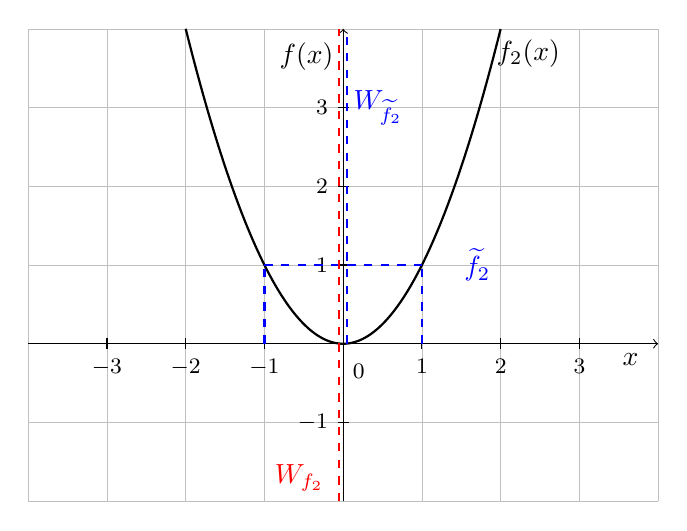
\begin{tikzpicture}
		
		% Gitternetzlinien
		\draw[xstep=1cm, ystep=1cm, very thin, color=lightgray] (-4,4) grid (4,-2);
		% x-Achse
		\draw[->] (-4,0) -- (4,0) node[below,xshift=-1em] {$x$}; 
		%Zahlen auf x-Achse
		\foreach \x in {-3,...,-1}
		\draw[shift={(\x,0)},color=black] (0pt,2pt) -- (0pt,-2pt) node[below] {\footnotesize $\x$};
		\foreach \x in {1,...,3}
		\draw[shift={(\x,0)},color=black] (0pt,2pt) -- (0pt,-2pt) node[below] {\footnotesize $\x$};
		% y-Achse 
		\draw[->] (0,-2) -- (0,4) node[left,yshift=-1em] {$f(x)$};%node[above left]
		%Zahlen auf y-Achse
		\foreach \y in {-1,...,-1}
		\draw[shift={(0,\y)},color=black] (2pt,0pt) -- (-2pt,0pt) node[left] {\footnotesize $\y$};
		\foreach \y in {1,...,3}
		\draw[shift={(0,\y)},color=black] (2pt,0pt) -- (-2pt,0pt) node[left] {\footnotesize $\y$};
		%Ursprung
		\draw[color=black] (0pt,-10pt) node[right] {\footnotesize $0$};
		
		
		
		\draw[thick,color=black] plot[samples=200, domain=-2:2] 
		(\x,{\x*\x}) node[below, xshift=1em]{$f_2(x)$};
		
		\draw[color=blue,thick,dashed] (-1,1) -- (1,1) node[xshift=2em] {$\widetilde{f}_2$};
		\draw[color=blue,thick,dashed] (-1,0) -- (-1,1);
		\draw[color=blue,thick,dashed] (1,0) -- (1,1);
		\draw[color=blue,thick,dashed] (0.05,0) -- (0.05,4);
		\draw[color=blue,thick,dashed] (0,3) node[right] {$\mathbb{W}_{\widetilde{f}_2}$};
		\draw[color=red,thick,dashed] (-0.05,-2) -- (-0.05,4);
		\draw[color=red,thick,dashed] (-1,-1.7) node[right] {$\mathbb{W}_{f_2}$};
	\end{tikzpicture}\\
\end{center}
\begin{quote}
	Nicht für jedes $ \textcolor{red}{y\in \mathbb{W}_{f_2}} $ existiert ein $x\in\mathbb{D}_{f_2}$, deswegen ist die Funktion nicht surjektiv.(z.B: $y=-1$)\\
	Für jedes $\textcolor{blue}{y\in\mathbb{W}_{\widetilde{f}_2}}$ existiert ein $x\in\mathbb{D}_{\widetilde{f}_2}$, deswegen ist die Funktion surjektiv.\\	
\end{quote}
Merke: Surjektivität hängt stark vom $\mathbb{W}_f$ ab.\vspace*{4mm}\\
\textbf{Definition (bijektiv):}\\
Eine Funktion $f:\mathbb{D}_f\longmapsto\mathbb{W}_f$ heißt bijektiv, wenn sie injektiv und surjektiv zugleich ist!\vspace*{2mm}\\
Merke:\\
Es gibt Funktionen, die weder injektiv noch surjektiv sind.\\
Beispiel: $f_2:\mathbb{R}\longmapsto\mathbb{R}$ mit $x\longmapsto x^2$ ist weder injektiv noch surjektiv.\\
\subsection{Aufgaben zur Injektivität und Surjektivität Teil I}

Überprüfe die folgende Funktion auf Injektivität und Surjektivität:
\begin{align*}
	f:\mathbb{R}\longmapsto\mathbb{R} \text{ mit } f(x)=(x-4)^3
\end{align*}
\textbf{Zur Injektivität}\\
Falls man weis, dass die Funktion nicht injektiv ist kann man ein Gegenbeispiel konstruieren.\\
Beweis der Injektivität:\\
Betrachte:\\ $f(x_1)=f(x_2)\Leftrightarrow (x_1-4)^3=(x_2-4)^3$\\
z.z: $x_1=x_2$\\
\underline{1.Fall:} $(x_1-4)\neq 0$\\
dann erhalten wir:\\
\begin{align*}
	\bigg(\frac{(x_2-4)}{(x_1-4)}\bigg)^3=1\Leftrightarrow\frac{(x_2-4)}{(x_1-4)}=1\Leftrightarrow x_2-4=x_1-4 \Leftrightarrow x_2=x_1
\end{align*} 
\underline{2.Fall:}$(x_1-4)=0\Leftrightarrow x_1=4$
\begin{align*}
	0=(x_1-4)^3=(x_2-4)^3=0\Leftrightarrow x_2=4\Leftrightarrow x_1=x_2
\end{align*}
\begin{align*}
	\text{also }x_1=x_{2_{\Square}}\text{    d.h. f ist injektiv}
\end{align*}
\subsection{Aufgaben zur Injektivität und Surjektivität Teil II}

\textbf{Zur Surjektivität}\\
Falls man weis, dass die Funktion nicht surjektiv ist kann man ein Gegenbeispiel konstruieren.\vspace*{2mm}\\
Beweis der Surjektivität:\\
Betrachte:\\ $f:\mathbb{R}\longmapsto\mathbb{R} \text{ mit } f(x)=(x-4)^3$\\
Sei $y\in\mathbb{R}$ beliebig. Es existiert ein $x\in\mathbb{R}$ mit $f(x)$ also mit $(x-4)^3=y$\vspace*{2mm}\\
Die Gleichung auf $x$ auflösen:\\
(Fallunterscheidung wegen negativer Wurzel)\\
\underline{1.Fall:} $y\in [0,\infty[$\\
\begin{quote}
	Betrachte:\\	
	$(x-4)^3=y\Leftrightarrow (x-4)=\sqrt[3]{y}\Leftrightarrow x=\sqrt[3]{y}+4\\$
\end{quote}
\begin{quote}
	Probe:\\
	$ f(x)=f(\sqrt[3]{y}+4)=((\sqrt[3]{y}+4)-4)^3=y$
\end{quote}
\underline{2.Fall:} $y\in \;]-\infty,0[$
\begin{quote}
	Betrachte:\\
	$(x-4)^3=y\Leftrightarrow-(-x+4)^3=y$\\
	Substituiere $y=-\widetilde{y}$\\
	$\Leftrightarrow-(-x+4)^3=-\widetilde{y}\Leftrightarrow(-x+4)^3=\widetilde{y}\Leftrightarrow -x+4=\sqrt[3]{\widetilde{y}}\Leftrightarrow x=-\sqrt[3]{\widetilde{y}}+4$
\end{quote}
\begin{quote}
	Probe:\\
	$f(x)=f(-\sqrt[3]{\widetilde{y}}+4)=((-\sqrt[3]{\widetilde{y}}+4)-4)^3=\big(-\sqrt[3]{\widetilde{y}\widetilde{y}}\big)^3=-\widetilde{y}=y_{_{\Square}}$
\end{quote}
Daraus folgt die Funktion ist surjektiv, und da die Funktion auch injektiv ist, ist die Funktion bijektiv.\\